\documentclass[11pt,a4paper]{article}
% ------------------------------------------------------------------
%  TP Docker - Containerisation & Orchestration (report)
% ------------------------------------------------------------------
\usepackage[utf8]{inputenc}
\usepackage[T1]{fontenc}
\usepackage{mathpazo}\usepackage{courier}
\usepackage[english]{babel}
\usepackage[a4paper,margin=2.0cm,top=2.2cm,bottom=2.2cm]{geometry}
\usepackage{graphicx}
\usepackage{xcolor}
\usepackage{listings}
\usepackage{booktabs}
\usepackage{tabularx}
\usepackage{fancyhdr}
\usepackage{titlesec}
\usepackage{caption}
\usepackage{enumitem}
\usepackage{float}
\usepackage{needspace}
\usepackage[most]{tcolorbox}
\usepackage{amssymb}
\usepackage{tikz}\usetikzlibrary{arrows.meta,positioning,fit,backgrounds,shapes.geometric}
\usepackage[hidelinks]{hyperref}

% ---------- colours ----------
\definecolor{accent}{HTML}{1D63ED}   % Docker blue
\definecolor{ink}{HTML}{1F2933}
\definecolor{soft}{HTML}{F3F6FA}
\definecolor{rule}{HTML}{C9D3E0}
\definecolor{kw}{HTML}{0B57D0}
\definecolor{cm}{HTML}{6B7785}
\definecolor{st}{HTML}{B3261E}

% ---------- headings ----------
\titleformat{\section}{\Large\bfseries\color{accent}}{\thesection}{0.8em}{}[\vspace{-0.6em}\color{rule}\rule{\textwidth}{0.6pt}]
\titleformat{\subsection}{\large\bfseries\color{ink}}{\thesubsection}{0.8em}{}
\titleformat{\subsubsection}{\normalsize\bfseries\color{ink}}{\thesubsubsection}{0.8em}{}
\setlength{\parindent}{0pt}
\setlength{\parskip}{0.45em}

% ---------- header / footer ----------
\pagestyle{fancy}
\fancyhf{}
\fancyhead[L]{\small\color{cm}TP Docker -- Containerisation \& Orchestration}
\fancyhead[R]{\small\color{cm}Student guide}
\fancyfoot[C]{\small\color{cm}\thepage}
\renewcommand{\headrulewidth}{0.4pt}

% ---------- captions ----------
\captionsetup{font=small,labelfont={bf,color=accent}}

% ---------- code listings ----------
\lstdefinestyle{tp}{
  basicstyle=\ttfamily\scriptsize\color{ink},
  backgroundcolor=\color{soft},
  frame=leftline, framerule=2pt, rulecolor=\color{accent},
  xleftmargin=6pt, framexleftmargin=6pt,
  keywordstyle=\color{kw}\bfseries,
  commentstyle=\color{cm}\itshape,
  stringstyle=\color{st},
  showstringspaces=false, breaklines=true, columns=fullflexible,
  numbers=left, numberstyle=\tiny\color{cm}, numbersep=8pt,
  literate={é}{{\'e}}1 {è}{{\`e}}1 {à}{{\`a}}1 {·}{{$\cdot$}}1 {→}{{$\rightarrow$}}1
}
\lstset{style=tp}
\lstdefinelanguage{Dockerfile}{
  morekeywords={FROM,AS,RUN,CMD,ENTRYPOINT,COPY,ADD,ENV,ARG,WORKDIR,USER,EXPOSE,VOLUME,LABEL,HEALTHCHECK},
  sensitive=true, morecomment=[l]{\#}, morestring=[b]"}
\lstdefinelanguage{yaml}{
  morekeywords={services,image,build,ports,volumes,networks,environment,depends_on,command,restart,profiles,name,driver,on,jobs,steps,uses,with,run,needs,runs-on,env,push,branches},
  sensitive=true, morecomment=[l]{\#}, morestring=[b]"}
\lstdefinelanguage{shell}{
  morekeywords={docker,compose,build,run,network,volume,create,inspect,images,ps,rm,push,tag,login,logs,exec,system,prune,curl},
  morecomment=[l]{\#}, morestring=[b]"}

% ---------- boxes ----------
\newtcolorbox{note}[1][]{colback=soft,colframe=accent,boxrule=0.6pt,arc=2pt,
  left=8pt,right=8pt,top=6pt,bottom=6pt,fonttitle=\bfseries\small,title=#1}
\newcommand{\shot}[3][0.78]{%
  \begin{figure}[H]\centering
  \fcolorbox{rule}{white}{\includegraphics[width=#1\textwidth]{screenshots/#2}}
  \caption{#3}\end{figure}}

% ==================================================================

% ---------------- title page ----------------

\newtcolorbox{tip}[1][]{colback=green!4,colframe=green!45!black,boxrule=0.6pt,arc=2pt,
  left=8pt,right=8pt,top=6pt,bottom=6pt,fonttitle=\bfseries\small,title=#1}
\newtcolorbox{warn}[1][]{colback=orange!6,colframe=orange!70!black,boxrule=0.6pt,arc=2pt,
  left=8pt,right=8pt,top=6pt,bottom=6pt,fonttitle=\bfseries\small,title=#1}
\tikzset{
  box/.style={draw=accent,rounded corners=3pt,fill=soft,align=center,font=\small,inner sep=6pt,minimum height=0.9cm},
  dbox/.style={draw=ink,rounded corners=3pt,fill=white,align=center,font=\small,inner sep=6pt,minimum height=0.9cm},
  arr/.style={-{Stealth[length=2.5mm]},thick,color=ink},
  lbl/.style={font=\scriptsize\itshape,color=cm}}

\begin{document}
\sloppy
\begin{titlepage}
\centering
\noindent\begin{minipage}[c]{0.17\textwidth}\raggedright\includegraphics[width=\linewidth]{screenshots/logo_insat.jpg}\end{minipage}%
\begin{minipage}[c]{0.62\textwidth}\centering\linespread{1.15}\selectfont
{\small\bfseries REPUBLIC OF TUNISIA}\\[2pt]
{\small Ministry of Higher Education and Scientific Research}\\[2pt]
{\small\bfseries University of Carthage}\\[2pt]
{\small\bfseries\color{accent} National Institute of Applied Sciences and Technology}
\end{minipage}%
\begin{minipage}[c]{0.21\textwidth}\raggedleft\includegraphics[width=\linewidth]{screenshots/logo_ucar.png}\end{minipage}\\[1.2cm]
{\color{accent}\rule{\textwidth}{1.2pt}}\\[0.8cm]
{\Huge\bfseries\color{ink} TP1 Docker -- Student Guide}\\[0.4cm]
{\Large\color{accent} Everything that was asked, everything that was done,\\[0.15cm] and how every file works}\\[0.8cm]
{\color{accent}\rule{\textwidth}{1.2pt}}\\[1.2cm]
\begin{tabular}{l}
\textbf{Group}\\[0.2cm]
Oussema \textsc{Bouchaala}\\ Mouin \textsc{El Dabbabi}\\ Mohamed Amin \textsc{Saddoud}\\ Mohamed Helmi \textsc{Lakhdhar}
\end{tabular}\\[1.4cm]
\begin{minipage}{0.82\textwidth}\small
This guide is a companion to the official lab report. The report \emph{proves} the work
(screenshots, analysis); this guide \emph{explains} it: what Docker concepts are involved,
what each file in the folder \texttt{TP1\_docker} does, and how to run everything again
yourself, step by step.
\end{minipage}
\vfill
{\small Generated on \today}
\end{titlepage}

\tableofcontents
\newpage

% =====================================================================
\needspace{14\baselineskip}
\section{The TP in one page}

\subsection{What was asked}
The TP has three parts. Part~A is the graded video tutorial; Part~B is the main lab
(an application called \emph{Visit-Counter}); Part~C automates everything with a pipeline.

\begin{center}
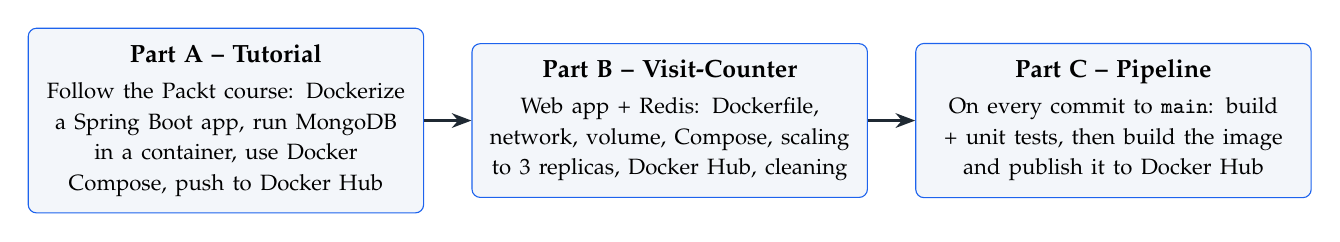
\begin{tikzpicture}[node distance=0.6cm and 0.6cm]
\node[box,text width=4.6cm] (a) {\textbf{Part A -- Tutorial}\\[2pt]\footnotesize Follow the Packt course: Dockerize a Spring Boot app, run MongoDB in a container, use Docker Compose, push to Docker Hub};
\node[box,text width=4.6cm,right=of a] (b) {\textbf{Part B -- Visit-Counter}\\[2pt]\footnotesize Web app + Redis: Dockerfile, network, volume, Compose, scaling to 3 replicas, Docker Hub, cleaning};
\node[box,text width=4.6cm,right=of b] (c) {\textbf{Part C -- Pipeline}\\[2pt]\footnotesize On every commit to \texttt{main}: build + unit tests, then build the image and publish it to Docker Hub};
\draw[arr] (a) -- (b); \draw[arr] (b) -- (c);
\end{tikzpicture}
\end{center}

\subsection{Checklist: requirement $\rightarrow$ where it is done}
{\small
\begin{tabularx}{\textwidth}{>{\raggedright\arraybackslash}p{6.3cm}>{\raggedright\arraybackslash}X c}
\toprule
\textbf{Requirement (TP statement)} & \textbf{Where / how} & \\
\midrule
Part 0: \texttt{docker version}, \texttt{docker login}, work folder & Docker Desktop 4.43.2; signed in as \texttt{oussemabouchaala}; folder \texttt{TP\_Docker\_Bouchaala\_\ldots} & \checkmark\\
P1: web app using Redis \texttt{db-service}, key \texttt{hits}, message with container ID & \texttt{partB-visit-counter/app/app.py} (Flask) & \checkmark\\
P1: Alpine/Slim base, non-root user, cache-friendly Dockerfile & \texttt{partB-visit-counter/Dockerfile} (\texttt{python:3.12-alpine}, \texttt{USER app}) & \checkmark\\
P1: \texttt{docker build -t counter-app:1.0 .} + size & 96.3~MB local, 22.4~MB on Docker Hub & \checkmark\\
P2: network \texttt{app-network}, volume \texttt{redis-data}, manual \texttt{docker run}, port 80 & commands in Section~\ref{sec:runB} & \checkmark\\
P2: robustness test (delete Redis, counter kept) & counter 8 $\rightarrow$ 9 after \texttt{docker rm -f} & \checkmark\\
P3: \texttt{docker-compose.yml} + \texttt{.env}, \texttt{--scale web=3}, analysis + load balancer & \texttt{docker-compose.yml}, \texttt{.env}, bonus \texttt{nginx/nginx.conf} & \checkmark\\
P4: tag + push to Docker Hub; one-command deep clean & \texttt{oussemabouchaala/counter-app}; \texttt{docker compose down --rmi all --volumes} & \checkmark\\
Report: commented Dockerfile, Compose, screenshots, RUN vs CMD, Hub link & \texttt{TP\_Docker\_Report\_\ldots pdf} (20 pages) & \checkmark\\
Part C: pipeline on each commit to \texttt{main}: tests, image build, push & \texttt{.github/workflows/ci-cd.yml} (GitHub Actions), runs \#2 and \#3 green & \checkmark\\
Part A: tutorial reproduced & \texttt{partA-tutorial/} (2 Spring Boot apps + MongoDB) & \checkmark\\
\bottomrule
\end{tabularx}}

\subsection{Important links}
\begin{note}[Online resources]
GitHub repository: \url{https://github.com/OussemaBouchaala/tp-docker-visit-counter}\\
Pipeline runs: \url{https://github.com/OussemaBouchaala/tp-docker-visit-counter/actions}\\
Docker Hub image: \url{https://hub.docker.com/r/oussemabouchaala/counter-app}
\end{note}

% =====================================================================
\needspace{14\baselineskip}
\section{Docker in 5 minutes (the concepts you need)}

\subsection{Image, container, registry}
\begin{center}
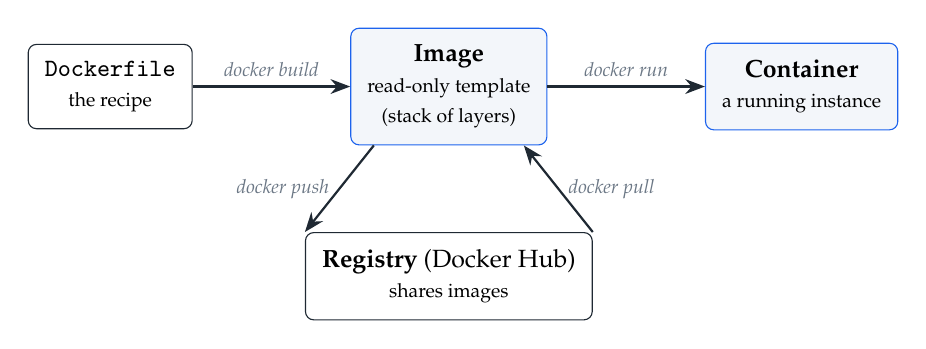
\begin{tikzpicture}[node distance=0.4cm and 2.0cm]
\node[dbox] (df) {\texttt{Dockerfile}\\\scriptsize the recipe};
\node[box,right=of df] (img) {\textbf{Image}\\\scriptsize read-only template\\\scriptsize (stack of layers)};
\node[box,right=of img] (c1) {\textbf{Container}\\\scriptsize a running instance};
\node[dbox,below=1.1cm of img] (hub) {\textbf{Registry} (Docker Hub)\\\scriptsize shares images};
\draw[arr] (df) -- node[above,lbl]{docker build} (img);
\draw[arr] (img) -- node[above,lbl]{docker run} (c1);
\draw[arr] (img.south west)++(0.3,0) -- node[left,lbl]{docker push} (hub.north west);
\draw[arr] (hub.north east) -- node[right,lbl]{docker pull} ([xshift=-0.3cm]img.south east);
\end{tikzpicture}
\end{center}

\begin{description}[leftmargin=1em,style=nextline]
\item[Image] A packaged application: code + runtime (Python, Java) + libraries + configuration. It is made of \emph{layers}: one per instruction of the Dockerfile. Layers are \textbf{cached}: if nothing changed, Docker reuses them (fast builds).
\item[Container] A running image. Each container has its own processes, file system, network address and hostname. Many containers can start from the same image (our 3 replicas).
\item[Registry] An image store. \texttt{docker push} uploads, \texttt{docker pull} downloads. Docker Hub is the public one.
\end{description}

\subsection{Network, volume, port mapping}
\begin{itemize}[leftmargin=1.3em]
\item \textbf{User-defined network}: containers on the same network can talk to each other \emph{by name} (Docker includes a small DNS server). That is why our app reaches Redis at the address \texttt{db-service}.
\item \textbf{Volume}: a storage area managed by Docker that \emph{survives} the container. A container's own files disappear with \texttt{docker rm}; the data in a volume stays.
\item \textbf{Port mapping} \texttt{-p HOST:CONTAINER}: makes a container port reachable from your PC. \texttt{-p 80:5000} means ``\texttt{http://localhost:80} on Windows goes to port 5000 inside the container''.
\end{itemize}

\subsection{Docker Compose}
Typing many \texttt{docker run} commands is error-prone. \textbf{Compose} describes the whole
application (services, networks, volumes, variables) in one YAML file, then
\texttt{docker compose up -d} starts everything and \texttt{docker compose down} removes it.

% =====================================================================
\needspace{14\baselineskip}
\section{The folder \texttt{TP1\_docker} file by file}

\begin{note}[Folder tree]
\scriptsize
\begin{verbatim}
TP1_docker/
|-- TP_Docker_Report_Bouchaala_ElDabbabi_Saddoud_Lakhdhar.pdf   <- official report (20 p.)
|-- TP1_Docker_Student_Guide.pdf                                 <- this guide
`-- TP_Docker_Bouchaala_ElDabbabi_Saddoud_Lakhdhar/             <- Git repository (on GitHub)
    |-- README.md                     project summary + pipeline badge
    |-- .gitignore                    files Git must ignore (caches, LaTeX temp files...)
    |-- .github/workflows/ci-cd.yml   PART C - the GitHub Actions pipeline
    |-- partA-tutorial/               PART A - projects from the video course
    |   |-- application-one/          Spring Boot "welcome" REST API
    |   |   |-- Dockerfile            multi-stage build (Maven -> JRE)
    |   |   |-- .dockerignore, pom.xml, mvnw, .mvn/   Maven build files
    |   |   |-- src/...               Java code (GreetingsController.java)
    |   |   `-- notes.txt             commands from the course
    |   |-- item-service-mongodb/     Spring Boot CRUD API + MongoDB
    |   |   |-- Dockerfile            same multi-stage pattern
    |   |   |-- docker-compose.yml    MongoDB + the API together
    |   |   `-- src/...               controllers, models, repositories
    |   `-- logs/                     real build logs (ignored by Git)
    |-- partB-visit-counter/          PART B - the Visit-Counter application
    |   |-- app/app.py                the Flask web service
    |   |-- app/requirements.txt      runtime libraries (Flask, redis, gunicorn)
    |   |-- requirements-dev.txt      + test libraries (pytest, fakeredis)
    |   |-- tests/test_app.py         4 unit tests (used by the pipeline)
    |   |-- Dockerfile                the image of the web service
    |   |-- .dockerignore             files NOT sent to the Docker build
    |   |-- docker-compose.yml        web + db-service (+ lb) orchestration
    |   |-- .env                      variables used by the Compose file
    |   `-- nginx/nginx.conf          bonus load balancer configuration
    `-- report/                       LaTeX source of the report
        |-- main.tex, main.pdf
        |-- screenshots/              all the real screenshots
        `-- code/                     copies of the files included in the report
\end{verbatim}
\end{note}

% =====================================================================
\needspace{14\baselineskip}
\section{Part B explained (the main lab)}

\subsection{Architecture}
\begin{center}
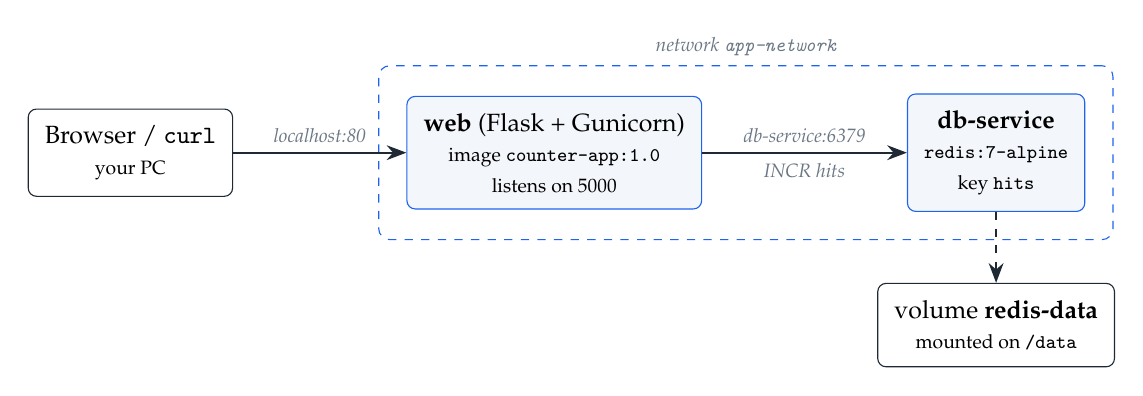
\begin{tikzpicture}[node distance=0.5cm and 1.0cm]
\node[dbox] (user) {Browser / \texttt{curl}\\\scriptsize your PC};
\node[box,right=2.2cm of user] (web) {\textbf{web} (Flask + Gunicorn)\\\scriptsize image \texttt{counter-app:1.0}\\\scriptsize listens on 5000};
\node[box,right=2.6cm of web] (db) {\textbf{db-service}\\\scriptsize \texttt{redis:7-alpine}\\\scriptsize key \texttt{hits}};
\node[dbox,below=0.9cm of db] (vol) {volume \textbf{redis-data}\\\scriptsize mounted on \texttt{/data}};
\draw[arr] (user) -- node[above,lbl]{localhost:80} (web);
\draw[arr] (web) -- node[above,lbl]{db-service:6379} node[below,lbl]{INCR hits} (db);
\draw[arr,dashed] (db) -- (vol);
\begin{scope}[on background layer]
\node[draw=accent,dashed,rounded corners,fit=(web)(db),inner sep=10pt,label={[lbl]above:network \texttt{app-network}}] {};
\end{scope}
\end{tikzpicture}
\end{center}

Each visit: the browser calls the web service $\rightarrow$ the service sends
\texttt{INCR hits} to Redis (atomic +1) $\rightarrow$ Redis returns the new value
$\rightarrow$ the page shows \emph{``Bonjour ! Cette page a été vue X fois. Je suis le conteneur [ID]''}.
Redis writes every change to its append-only file in the volume, so the number survives.

\subsection{\texttt{app/app.py} -- the web service}
\lstinputlisting[language=Python,linerange={7-20,40-76}]{code/app.py}
\begin{itemize}[leftmargin=1.3em]
\item Lines 7--20: read \texttt{REDIS\_HOST} (default \texttt{db-service}) and \texttt{REDIS\_PORT} from the environment and create a Redis client.
\item \texttt{get\_hit\_count()}: \texttt{client.incr("hits")} adds 1 and returns the new value. If Redis is restarting it waits 0.5~s and retries up to 5 times -- this is what makes the robustness test smooth.
\item \texttt{container\_id()}: inside Docker, the \emph{hostname} of a container is its short ID, so \texttt{socket.gethostname()} gives the ``Je suis le conteneur [ID]'' part.
\item \texttt{index()} (route \texttt{/}): builds the message and puts it in a small HTML page; if Redis is unreachable it answers HTTP~503.
\item \texttt{health()} (route \texttt{/health}): a simple check used by the tests.
\end{itemize}

\subsection{\texttt{Dockerfile} -- line by line}
\lstinputlisting[language=Dockerfile]{code/Dockerfile}
\begin{center}\small
\begin{tabularx}{\textwidth}{lX}
\toprule
\textbf{Instruction} & \textbf{Why}\\
\midrule
\texttt{FROM python:3.12-alpine} & Smallest official Python base (Alpine Linux $\approx$7~MB).\\
\texttt{ENV \ldots} & No \texttt{.pyc} files, logs printed immediately (visible in \texttt{docker logs}).\\
\texttt{RUN addgroup/adduser} & Creates the unprivileged user \texttt{app} (security).\\
\texttt{COPY requirements.txt} then \texttt{RUN pip install} & \textbf{Cache trick}: dependencies change rarely, so this slow layer is reused when only the code changes.\\
\texttt{COPY app/ .} & The code, copied last because it changes often.\\
\texttt{USER app} & From here on, the container does not run as root.\\
\texttt{EXPOSE 5000} & Documents the port the app listens on.\\
\texttt{CMD gunicorn \ldots} & Default start command: a production web server with 2 workers.\\
\bottomrule
\end{tabularx}
\end{center}

\begin{tip}[RUN vs CMD in one sentence]
\texttt{RUN} executes \emph{during the build} and saves the result in the image;
\texttt{CMD} is executed \emph{each time a container starts}.
\end{tip}

\texttt{.dockerignore} lists files that must not be copied into the image
(\texttt{tests/}, \texttt{.env}, caches, \texttt{.git}\ldots): smaller, safer build context.

\subsection{Manual deployment (Part 2)}\label{sec:runB}
\begin{lstlisting}[language=shell]
docker build -t counter-app:1.0 .                 # 1. build the image
docker network create app-network                 # 2. private network
docker volume create redis-data                   # 3. persistent storage
docker run -d --name db-service --network app-network \
       -v redis-data:/data redis:7-alpine redis-server --appendonly yes
docker run -d --name web-app --network app-network -p 80:5000 counter-app:1.0
# open http://localhost  ->  "Bonjour ! Cette page a ete vue 1 fois ..."
docker rm -f db-service                           # robustness test: kill Redis
docker run -d --name db-service --network app-network \
       -v redis-data:/data redis:7-alpine redis-server --appendonly yes
# refresh: the counter continues (data was in the volume)
\end{lstlisting}

\shot[0.7]{08_robustness.png}{Real output of the robustness test: 8 visits, Redis deleted and recreated, next visit is 9.}

\subsection{\texttt{docker-compose.yml} and \texttt{.env} (Part 3)}
\lstinputlisting[language=yaml,firstline=6]{code/docker-compose.yml}
\begin{itemize}[leftmargin=1.3em]
\item \texttt{\$\{APP\_PORT\}}, \texttt{\$\{WEB\_HOST\_PORTS\}}\ldots{} are replaced by the values of the \texttt{.env} file sitting next to the YAML: no port is written ``in hard''.
\item \texttt{web} has no \texttt{container\_name}: Docker must be free to create \texttt{web-1}, \texttt{web-2}, \texttt{web-3}.
\item \texttt{depends\_on}: Redis is started before the web service.
\item \texttt{restart: unless-stopped}: containers restart automatically (e.g.\ after a reboot).
\item The \texttt{lb} service has \texttt{profiles: ["lb"]}: it is only started when we add \texttt{--profile lb}.
\end{itemize}
\lstinputlisting[language=shell]{code/env.txt}

\subsection{Scaling: why 3 replicas cannot share port 80}
\begin{center}
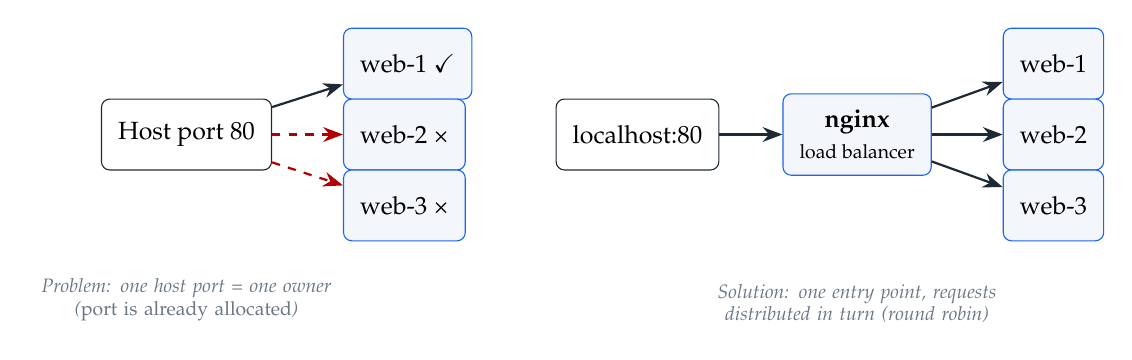
\begin{tikzpicture}[node distance=0.35cm and 0.9cm]
% problem
\node[dbox] (h) {Host port 80};
\node[box,right=of h,yshift=0.9cm] (w1) {web-1 \checkmark};
\node[box,right=of h] (w2) {web-2 \texttimes};
\node[box,right=of h,yshift=-0.9cm] (w3) {web-3 \texttimes};
\draw[arr] (h) -- (w1); \draw[arr,red!70!black,dashed] (h) -- (w2); \draw[arr,red!70!black,dashed] (h) -- (w3);
\node[lbl,below=1.25cm of h,text width=3.8cm,align=center] {Problem: one host port = one owner\\ (\emph{port is already allocated})};
% solution
\node[dbox,right=3.6cm of h] (u) {localhost:80};
\node[box,right=0.8cm of u] (lb) {\textbf{nginx}\\\scriptsize load balancer};
\node[box,right=0.9cm of lb,yshift=0.9cm] (r1) {web-1};
\node[box,right=0.9cm of lb] (r2) {web-2};
\node[box,right=0.9cm of lb,yshift=-0.9cm] (r3) {web-3};
\draw[arr] (u) -- (lb); \draw[arr] (lb) -- (r1); \draw[arr] (lb) -- (r2); \draw[arr] (lb) -- (r3);
\node[lbl,below=1.25cm of lb,text width=4.2cm,align=center] {Solution: one entry point, requests distributed in turn (round robin)};
\end{tikzpicture}
\end{center}

A TCP port of the Windows host can only be opened by one program. The first replica
takes port 80, the two others fail. Two solutions were implemented:
(1) a \textbf{port range} \texttt{8081-8083} (one port per replica, from \texttt{.env});
(2) a \textbf{load balancer}: \texttt{nginx} alone owns port 80 and forwards each request to one
of the replicas through the internal network.

\lstinputlisting{code/nginx.conf}
\texttt{server web:5000} is enough because Docker's DNS returns the IP addresses of
\emph{all} replicas of the service \texttt{web}; \texttt{zone} shares the round-robin
counter between nginx processes so that requests really alternate.

\shot[0.72]{12_lb_round_robin.png}{Real output: 6 requests on \texttt{localhost:80} answered in turn by the 3 containers.}

\subsection{Publication and cleaning (Part 4)}
\begin{lstlisting}[language=shell]
docker tag  counter-app:1.0 oussemabouchaala/counter-app:1.0   # name = user/repo:tag
docker push oussemabouchaala/counter-app:1.0
docker compose --profile lb down --rmi all --volumes --remove-orphans   # deep clean
\end{lstlisting}
\begin{warn}[Why not \texttt{docker system prune -a --volumes}?]
That command cleans the \emph{whole} computer: it would also have deleted the volumes
of other projects on the laptop (Odoo, PostgreSQL). The Compose command only removes
what this project created: containers, network, images and volume.
\end{warn}

\subsection{\texttt{tests/test\_app.py} -- unit tests}
\lstinputlisting[language=Python,linerange={1-30}]{code/test_app.py}
\texttt{fakeredis} is an in-memory imitation of Redis, so the tests run anywhere (even
in GitHub's servers) without a real database. The 4 tests check: the counter
increments (1 then 2), the message contains the container ID, \texttt{/health}
returns \texttt{ok}, and the app answers 503 when Redis is down.

% =====================================================================
\needspace{14\baselineskip}
\section{Part A explained (the tutorial)}

\begin{center}
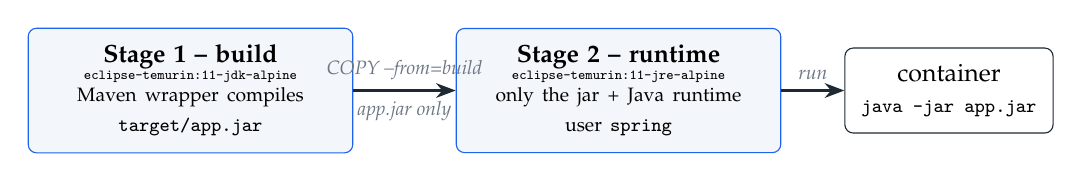
\begin{tikzpicture}[node distance=0.4cm and 1.0cm]
\node[box,text width=3.7cm] (s1) {\textbf{Stage 1 -- build}\\\tiny \texttt{eclipse-temurin:11-jdk-alpine}\\\scriptsize Maven wrapper compiles\\\scriptsize \texttt{target/app.jar}};
\node[box,right=1.3cm of s1,text width=3.7cm] (s2) {\textbf{Stage 2 -- runtime}\\\tiny \texttt{eclipse-temurin:11-jre-alpine}\\\scriptsize only the jar + Java runtime\\\scriptsize user \texttt{spring}};
\node[dbox,right=0.8cm of s2] (c) {container\\\scriptsize \texttt{java -jar app.jar}};
\draw[arr] (s1) -- node[above,lbl]{COPY --from=build} node[below,lbl]{app.jar only} (s2);
\draw[arr] (s2) -- node[above,lbl]{run} (c);
\end{tikzpicture}
\end{center}

\begin{itemize}[leftmargin=1.3em]
\item \textbf{application-one}: a Spring Boot REST API, \texttt{GET /api/v1/welcome}. Run with
\texttt{docker run -p 8090:8080 application-one-img:v1}.
\item \textbf{item-service-mongodb}: a CRUD API on \texttt{/api/v1/items} that stores items in MongoDB.
\item In the course, the jar was built on the PC and copied with \texttt{FROM openjdk:11 / ADD target/app.jar}.
We used a \textbf{multi-stage build} instead: no Java or Maven needed on the PC, the deprecated
\texttt{openjdk} image is avoided, and the final image contains no build tools.
\end{itemize}

\lstinputlisting[language=yaml,caption={\texttt{partA-tutorial/item-service-mongodb/docker-compose.yml}}]{code/compose.partA.yml}
The application finds MongoDB by the service name \texttt{mongodb-container-one}; the
environment variables \texttt{SPRING\_DATA\_MONGODB\_HOST/PORT} override the values written
in \texttt{application-local.properties} (which pointed to \texttt{host.docker.internal:28000}).

\shot[0.7]{A4_crud_mongo.png}{Real test: two items created with \texttt{POST} (201), listed with \texttt{GET}, and found inside MongoDB with \texttt{mongosh}.}

% =====================================================================
\needspace{14\baselineskip}
\section{Part C explained (the CI/CD pipeline)}

\begin{center}

\begin{tikzpicture}[node distance=0.4cm and 0.8cm]
\node[dbox] (dev) {\texttt{git push}\\\scriptsize branch \texttt{main}};
\node[box,right=of dev,text width=3.2cm] (j1) {\textbf{Job 1}\\\scriptsize install, syntax check,\\\scriptsize \texttt{pytest} (4 tests)};
\node[box,right=of j1,text width=3.3cm] (j2) {\textbf{Job 2} (if Job 1 OK)\\\scriptsize login with secrets,\\\scriptsize build \& push image};
\node[dbox,right=of j2] (hub) {Docker Hub\\\scriptsize \texttt{:latest}, \texttt{:<sha>}};
\draw[arr] (dev) -- (j1); \draw[arr] (j1) -- node[above,lbl]{needs} (j2); \draw[arr] (j2) -- (hub);
\end{tikzpicture}
\end{center}

\lstinputlisting[language=yaml,firstline=10]{code/ci-cd.yml}

\begin{itemize}[leftmargin=1.3em]
\item \texttt{on: push: branches: ["main"]}: GitHub starts the workflow automatically on every commit pushed to \texttt{main}.
\item \texttt{runs-on: ubuntu-latest}: GitHub provides a fresh Linux machine for each job (nothing to install, unlike Jenkins).
\item \texttt{needs: build-and-test}: the image is published \emph{only} if the tests passed.
\item \texttt{secrets.DOCKERHUB\_USERNAME / DOCKERHUB\_TOKEN}: encrypted values stored in the repository settings -- the password is never written in the code.
\item Two tags: \texttt{latest} (newest version) and the commit SHA (to know exactly which code an image contains, and to roll back).
\end{itemize}

\begin{tip}[What happened in our runs]
Run \#1 failed at \emph{Log in to Docker Hub} because the secrets did not exist yet (tests
had passed). After adding them, runs \#2 and \#3 were fully green and the images
appeared on Docker Hub.
\end{tip}

\shot[0.55]{C1_actions_runs.png}{The pipeline runs on GitHub Actions.}

% =====================================================================
\needspace{14\baselineskip}
\section{How to run everything again (cheat sheet)}
Open a PowerShell (or the Docker Desktop terminal) in the project folder.

\subsection*{Part B}
\begin{lstlisting}[language=shell]
cd partB-visit-counter
docker build -t counter-app:1.0 .
docker compose up -d --scale web=3                 # replicas on 8081, 8082, 8083
docker compose --profile lb up -d --scale web=3    # + load balancer on http://localhost
docker compose ps                                   # what is running
docker compose logs -f                              # live logs (Ctrl+C to quit)
docker exec -it visit-counter-web-1 sh              # enter a container
docker compose --profile lb down --rmi all --volumes --remove-orphans   # clean
\end{lstlisting}

\subsection*{Part A}
\begin{lstlisting}[language=shell]
cd partA-tutorial\application-one
docker build -t application-one-img:v1 .
docker run -d -p 8090:8080 --name app1 application-one-img:v1
curl http://localhost:8090/api/v1/welcome
cd ..\item-service-mongodb
docker compose up -d                                # MongoDB + item-service
curl http://localhost:8090/api/v1/items
docker compose down --volumes
\end{lstlisting}

\subsection*{Unit tests without Docker}
\begin{lstlisting}[language=shell]
cd partB-visit-counter
pip install -r requirements-dev.txt
pytest -v
\end{lstlisting}

\subsection*{Part C}
Edit any file, commit, then \textbf{Push origin} in GitHub Desktop: the pipeline starts by
itself (tab \emph{Actions} of the repository).

\begin{warn}[Practical problems we met (and the fix)]
\begin{itemize}[leftmargin=1.2em]
\item \textbf{Slow Internet}: downloading the Maven, JDK and MongoDB images took $\approx$20~min. Pull images once, then everything comes from the cache.
\item \textbf{Docker Desktop terminal froze} on the animated progress bars of Compose. Fix: add \texttt{--ansi never --progress plain}.
\item \textbf{nginx always chose the same replica}: each nginx worker had its own round-robin counter; fixed with \texttt{zone visit\_counter 64k;}.
\item \textbf{Garbled accents} in PowerShell (\texttt{é} instead of \texttt{é}): \texttt{[Console]::OutputEncoding = [Text.Encoding]::UTF8}.
\end{itemize}
\end{warn}

% =====================================================================
\needspace{14\baselineskip}
\section{Glossary}
\begin{center}\small
\begin{tabularx}{\textwidth}{lX}
\toprule
Alpine & Very small Linux distribution used as a base image.\\
Bridge network & Default type of Docker network on one machine; user-defined bridges add DNS by name.\\
Build context & The files sent to Docker by \texttt{docker build .} (filtered by \texttt{.dockerignore}).\\
CI/CD & Continuous Integration / Continuous Delivery: automatic test and delivery on each change.\\
Gunicorn & Production web server for Python applications.\\
Layer & One step of an image; layers are cached and shared between images.\\
Load balancer & Single entry point that spreads requests across several replicas.\\
Multi-stage build & Dockerfile with several \texttt{FROM}: build in one stage, copy only the result into a small final image.\\
Redis & In-memory key-value database; \texttt{INCR} increments a number atomically.\\
Replica & One of several identical containers of the same service.\\
Secret & Encrypted value stored by GitHub (tokens, passwords) usable by the pipeline.\\
Volume & Docker-managed storage that outlives containers.\\
\bottomrule
\end{tabularx}
\end{center}

\end{document}
